
\documentclass{article}

\usepackage{graphicx}
\usepackage{tabularx}
\author{Allen Hsu, Kevin A. Wortman}

\begin{document}

\title{FCL: A Functional Domain-specific Embedded Language for GPU Programming}

\date{}

\begingroup
\let\center\flushleft
\let\endcenter\endflushleft
\maketitle
\endgroup

{\raggedright{}
\noindent
Abstract. We propose a Functional Programming language for utilizing the Graphics
Processing Unit for General Purpose Computation. General Purpose Programming
on the GPU (GPGPU) has been a long sought after endeavor; the number of threads
available on a GPU vastly outnumber the number of threads on a CPU. However
due to the difficulties of programming for the GPU, this potential has been
largely untapped. FCL is our attempt at making the programming process much
simpler, both syntactically and algorithmically. Because of the inherent
statelessness of parallelization, we believe a functional language is the most
appropriate. Functional Programming is inherently stateless; where an
algorithm written for a sequential environment would be exactly the same as one
written for an parallel environment.
}

\section{\emph{Introduction}}

\paragraph{}

The future of computing is parallel processing. As clock speeds will eventually
max out and the only way to improve speeds is with a larger quantity of threads.
Most applications in the software industry are not optimized to use parallel
processing. Applications that do take advantage of parallel processing can be
optimized further by processing their computation on a GPU rather than a CPU.

The main obstacle impeding programmers from attempting general purpose GPU
computing is the difficulty of implementation. All GPGPU APIs at the moment are
written in low level languages such as C, C++, and Fortran; the most notable ones
being CUDA and OpenCL. The difficulty, or
more accurately tediousness, of the steps required to use these APIs can be avoided.
Wrapping these APIs in high level languages such as Haskell or Python
have been attempted before. However, the problem with theses attempts is that they
still follow the same workflow as the original low level APIs. They are simply
extensions meant to allow access to CUDA or OpenCL, rather than offering true
higher level abstraction.

Our answer to this problem is FCL. FCL is a domain-specific embedded language in
Chicken Scheme. FCL allows one to write in a high level functional language, based
 on Scheme, that compiles into OpenCL kernel code. Next, FCL offers powerful
control procedures for applying these `kernels' onto CPU memory. We believe that
the low level operations of transferring data from buffer to buffer,
device to device, or vice versa should be abstracted away from the programmer.
That will allow the programmer more freedom to solve bigger and more dynamic problems.

\section{Overview}

\subsection{Domain-specific language}
\paragraph{}
A domain-specific language, commonly referred to as a DSL, is a language designed
for a specific purpose in a specific domain. Embedded variants of DSLs are
extensions of the parent language and are implemented as a library. The purpose
 of FCL is to make creating a GPU accelerated program to be as simple as creating a normal
single threaded CPU program and the domain of the language is Chicken Scheme.

\subsection{Functional Paradigm}
To unify non-parallel and parallel code, we chose the Functional Paradigm.
Functional code is written in a way that is stateless and not dependent on
execution order. If a program were written in a functional manner parallelization
would essentially be painless. In contrast, when programs are written in a non-functional way, they
usually are inherently full of state and rely on sequential execution. When an
program is dependent on variable states and execution order, it is not naturally
parallelizable. Having stateless code allows a program to be made parallel without
modification, which means parallel and non-parallel code would look exactly the
same.

\subsection{Chicken Scheme}
Chicken is a compiler for the Scheme programming language;
Chicken produces very portable and efficient C. What is unique about Chicken is
that it has a very powerful foreign function interface for embedding C code. It
is for this reason we chose Chicken over other implementations of Scheme. The
foreign function interface allows us to include the OpenCL library directly into
our FCL library and call its functions.

\subsection{OpenCL}
\paragraph{}
The back end to FCL is OpenCL. In fact, the name FCL is a reference OpenCL.
The `CL' comes from OpenCL and stands for `Computing Language' and the `F' stands
for `Functional', in total `Functional Computing Language'. We chose OpenCL because
of its portability and Open Source nature.  OpenCL is an API framework for
creating programs that utilize parallelization on either a CPU or GPU. It offers
a C99 based language for writing kernels and a robust C language API
for transferring data from a host program to a parallelization platform.
In OpenCL there is a device scope and an host scope. An OpenCL
program can be briefly described as a program that takes a kernel defined in the device scope and
 maps it to data buffers allocated on the host scope. This mapping is done in parallel,
where the kernel is run N times (N represents number of items in the buffer). After
the kernel has been applied to the buffer, the result is then transferred back to
the host scope and can be then used in other operations.

%% Not sure whether or not to explain the OpenCL programming process
%% In order to create an OpenCL program, one must follow a series of tedious procedures. The
%% programmer first needs to create a reference to a GPU device. Then create a
%% context on the referenced device. Next, the programmer needs to provide source
%% code in the form of OpenCL C. This source code is then compiled into a kernel,
%% which is then attached to a OpenCL program. Finally the program is ready to be
%% run with input and output buffers. However, the steps to setup input and output
%% buffers are just as tedious. The programmer must allocate memory on the CPU
%% and allocate memory on the GPU, then transfer the data from the CPU buffer onto
%% the GPU buffer. To run the previously set up OpenCL program with these inputs
%% and outputs, the programmer then maps the GPU buffers as arguments to the
%% kernel. After all computation is done the programmer must also remember to
%% deallocate both the CPU buffers and GPU buffers.

\subsection{FCL Scope}
\paragraph{}
FCL, like OpenCL, has two scopes; the device scope and the host scope.
The device scope resides on the parallel processing unit, i.e. the GPU.
The host scope resides on the CPU, in the same scope as all normal scheme code.
FCL keywords for defining things in the device scope are indicated with a
`g' as its first letter, e.g. gdefine, glambda, etc. The `g' scope is
compiled by the FCL compiler into OpenCL kernel source code and then loaded
onto an OpenCL kernel program.  The kernel program can then be invoked using
host scope command procedures, i.e. pmap, pfilter, and `g' data types, i.e.
gdata, gbuffer. The FCL kernel compilation does not disrupt the compile process of
Chicken Scheme because the kernel compilation occurs at run time. Essentially
there are 2 compilations and 2 runs. First there is the host code compilation and run
time. Then there is the device code compilation and run time that occurs within
the host's run time.

\subsection{FCL Compilation}
\paragraph{}
FCL is a true embedded language. Meaning it is included like any other library
in Scheme and the program is only manually compiled once by the user.

\subsection{FCL Typing}
\paragraph{}
FCL is a strongly typed language. All variables upon initialization must have a
type specification.

\section{\emph{Description}}
\subsection{Fundamental Types}

\raggedright{}{
  {\emph{Base}}:
}

\begin{quote}
\begin{verbatim}
bool, char, short, int, float, double, record
\end{verbatim}
\end{quote}

\raggedright{}{
  {\emph{Unsigned}}:
}

\begin{quote}
\begin{verbatim}
uchar, ushort, uint
\end{verbatim}
\end{quote}

\raggedright{}{
{\emph{List}}
}
\begin{quote}
\begin{verbatim}
bool*, char*, short*, int*, float*, double*, record*
\end{verbatim}
\end{quote}

\subsection{Functions}

\raggedright{}{
{\emph{Standard Definition}}
}
\begin{quote}
\begin{verbatim}
(gdefine add (glambda ((int x) (int y) -> int)
               (g+ x y)))

(gdefine sin-1 (glambda (int)
                 (gsin 1)))
\end{verbatim}
\end{quote}

\raggedright{}{
{\emph{Syntactic Sugar Definition}}
}
\begin{quote}
\begin{verbatim}
(gdefine (add (int x) (int y) -> int)
  (g+ x y))

(gdefine (sin-1 -> int)
  (gsin 1))

\end{verbatim}
\end{quote}

\raggedright{}{
{\emph{Syntactic Sugar Definition, marked for early compilation}}
}
\begin{quote}
\begin{verbatim}
(gdefine* (add (int x) (int y) -> int)
  (g+ x y))

(gdefine* (sin-1 -> int)
  (gsin 1))

\end{verbatim}
\end{quote}

\subsection{Conditional Statements}

\raggedright{}{
{\emph{if}}
}
\begin{quote}
\begin{verbatim}
(gdefine (minimum (int x) (int y) -> int)
  (gif (g> x y)
       x
       y))

(minimum 4 3)  ; returns 3
(minimum 2 10) ; returns 2

\end{verbatim}
\end{quote}

\raggedright{}{
{\emph{cond}}
}
\begin{quote}
\begin{verbatim}
(gdefine (clamp (int x) (int min) (int max) -> int)
  (gcond ((g< min x) min)
         ((g> max x) max)
         (else x)))

(clamp 4 1 10) ; returns 4
(clamp 3 5 10) ; returns 5

\end{verbatim}
\end{quote}

\raggedright{}{
{\emph{case}}
}
\begin{quote}
\begin{verbatim}
(gdefine (grade (int x) -> char)
  (gcase x
    ((4) "A")
    ((3) "B")
    ((2) "C")
    ((1) "D")
    (else "F")))

(gdefine (tier (char g) -> int)
  (gcase g
    (("A" "B") 1)
    (("C" "D") 2)
    (("F") 3)
    (else 4)))

(grade 4)        ; returns "A"
(grade 2)        ; returns "C"
(grade 0)        ; returns "F"
(grade -1)       ; returns "F"
(tier (grade 2)) ; returns 2
(tier (grade 4)) ; returns 1
(tier 10)        ; returns 4

\end{verbatim}
\end{quote}

\subsection{Lists}
\raggedright{} {
{\emph{Standard Initialization}}
}

\begin{quote}
\begin{verbatim}
(gdefine lst (glist int 1 2 3 4 5 6 7 8 9 10))
\end{verbatim}
\end{quote}

\raggedright{} {
{\emph{Conversion Initialization}}
}

\begin{quote}
\begin{verbatim}
(gdefine lst (list->glist int (list 1 2 3 4 5 6 7 8 9 10)))
\end{verbatim}
\end{quote}

\subsection{Higher-order Expressions}

{\emph{Map}}
\begin{quote}
\begin{verbatim}
(gdefine (square (int x) -> int)
  (* x x))

(define result (gmap square (glist int 1 2 3 4 5)))

;; result returns (glist int 1 4 9 16 25)

\end{verbatim}
\end{quote}

{\emph{Fold}}
\begin{quote}
\begin{verbatim}
(gdefine (find-largest (int* lst) -> int)
  (gfold (glambda ((int curr) (int prev) -> int)
           (gif (g> curr prev)
                curr
                prev))
         0
         lst))

(find-largest (glist int 1 2 3 4 5 6 7 8 9)) ; returns 9
\end{verbatim}
\end{quote}

\subsection{Embedding Scheme}

\raggedright{}{
{\emph{Scheme Procedures (behave like macros in FCL `g' namespace)}}
}

\begin{quote}
\begin{verbatim}
(define (formula a b)
  (g/ (g+ a b) 2))

(gdefine (foo1 (float x) (float y) -> float)
  (formula x y))

;; equivalent to foo1
(gdefine (foo2 (float x) (float y) -> float)
  (g/ (g+ x y) 2))

(define (sum-list a)
  (fold + 0 a))

(gdefine (foo3 (float x) -> float)
  (g+ (sum-list (list 1 2 3 4 5)) x))

;; equivalent to foo3
(gdefine (foo4 (float x) -> float)
  (g+ 15 x))
\end{verbatim}
\end{quote}

\subsection{Objects}

\raggedright{}{
{\emph{Record Types}}
}

\begin{quote}
\begin{verbatim}
(gdefine-record-type <vec>
  (vec (float x) (float y) (float z))
  (x vec-x)
  (y vec-y)
  (z vec-z))

(gdefine-record-type <triangle>
  (triangle (vec v0) (vec v1) (vec v2))
  (v0 triangle-v0)
  (v1 triangle-v1)
  (v2 triangle-v2))

(gdefine-record-type <sphere>
  (sphere (vec pos) (float radius))
  (pos sphere-pos)
  (radius sphere-radius))
\end{verbatim}
\end{quote}

\begin{quote}
\begin{verbatim}
(gdefine vec1 (vec 1.0 3.2 1.0))
(gdefine vec2 (vec 4.0 2.1 3.5))
(gdefine vec3 (vec 9.9 2.4 3.0))
(gdefine a-sphere (sphere vec1 5.0))
(gdefine a-triangle (triangle vec1 vec2 vec3))

(sphere-pos a-sphere)    ; accesses pos property of a-sphere
(triangle-v0 a-triangle) ; accesses v0 property of a-triangle
\end{verbatim}
\end{quote}

\subsection{Polymorphism}
{\emph{Compile Time Selection}}

\begin{quote}
\begin{verbatim}
(gdefine (gmember-int? (int value) (int* lst) -> bool)
  (gfold (glambda ((int curr) (int prev) -> int)
           (gif (g= curr value)
                gtrue
                prev))
         gfalse
         lst))

(gdefine (gmember-float? (float value) (float* lst) -> bool)
  (gfold (glambda ((float curr) (float prev) -> float)
           (gif (g= curr value)
                gtrue
                prev))
         gfalse
         lst))

(gdefine (gmember-double? (double value) (double* lst) -> bool)
  (gfold (glambda ((double curr) (double prev) -> double)
           (gif (g= curr value)
                gtrue
                prev))
         gfalse
         lst))

(define gmember-dictionary
  (list (cons "int" gmember-int?)
        (cons "float" gmember-float?)
        (cons "double" gmember-double?)))

(define (gmember-poly type)
  (cdr (assoc type gmember-dictionary)))

(define (gmember? value lst)
  ((gmember-poly (gtype lst)) value lst))

\end{verbatim}
\end{quote}

{\emph{Run Time Selection}}

\begin{quote}
\begin{verbatim}
(gdefine (intersect? (record obj) (ray r) -> bool)
  (gcond ((sphere? obj) (sphere-intersect? obj r))
         ((triangle? obj) (triangle-intersect? obj r))
         (else gfalse)))
\end{verbatim}
\end{quote}


\subsection{Intermediate Objects}

{\emph{Lists}}

\begin{quote}
\begin{verbatim}
(define buffer (list->gbuffer int (iota 1000)))

;; usable with FCL parallel higher order functions
(define new-buffer (pmap gfoo buffer))

;; accessible within gprocedures
(gdefine (can-use-buffer (int x) -> int)
  (g+ x (gfold + 0 buffer)))

\end{verbatim}
\end{quote}

{\emph{Atoms}}

\begin{quote}
\begin{verbatim}
(define data (gdata int 100))

;; accessible within gprocedures
(gdefine (can-use-data (int x) -> int)
  (g+ x data))

\end{verbatim}
\end{quote}

{\subsection{Parallel Higher-Order Expressions}

{\emph{Map}}
\begin{quote}
\begin{verbatim}
(gdefine* (double (int x) -> int)
  (g+ x x))

(pmap double (list->gbuffer int (list 1 2 3 4 5)))
;; returns a gbuffer containing (2 4 6 8 10)
\end{verbatim}
\end{quote}

{\emph{Filter and Remove}}

\begin{quote}
\begin{verbatim}
(gdefine* (even? (int x) -> bool)
  (g= (gmodulo x 2) 0))

(define buffer (list->gbuffer int (list 1 2 3 4 5)))

(pfilter even? buffer) ; returns gbuffer with (2 4)
(premove even? buffer) ; returns gbuffer with (1 3 5)
\end{verbatim}
\end{quote}

\subsection{FCL Procedures}

{\emph{FCL Context}}
\begin{quote}
\begin{verbatim}
(fcl-begin) ; allocates and initializes a FCL context on the GPU device

#| your code would be here |#

(fcl-end)   ; releases FCL context and any unfreed intermediate objects
\end{verbatim}
\end{quote}

{\emph{FCL Expressions}}
\begin{quote}
\begin{verbatim}
(define-fcl-exp (run-gpu-code n)
  (define buffer (list->gbuffer int (iota n)))

  (gdefine* (double (int x) -> int)
    (g+ x x))

  (gbuffer->list (pmap double buffer)))

;; FCL expressions ensure that all gprocedures, gbuffers and gdata defined
;; within it are released when it goes out of scope.
\end{verbatim}
\end{quote}

\subsection{Simple Example}

{\raggedright{}
First we must allocate and initialize a FCL context.
}
\begin{quote}
\begin{verbatim}
(fcl-begin)
\end{verbatim}
\end{quote}

{\raggedright{}
Next lets create a simple gprocedure that adds two integers.
}

\begin{quote}
\begin{verbatim}
(gdefine* (gadd-nums (int x) (int y) -> int)
  (g+ x y))
\end{verbatim}
\end{quote}

{\raggedright{}
Notice we use gdefine* for gadd-nums instead of the normal gdefine. This will mark this gprocedure
to be compiled and loaded onto the gpu as soon as it is defined; otherwise compilation
would occur when the
gprocedure is used in host scope or explicitly included using fcl-include.
An equivalent procedure to gadd-nums in the host scope would be
}

\begin{quote}
\begin{verbatim}
(define (add-nums x y)
  (+ x y))
\end{verbatim}
\end{quote}

{\raggedright{}
One way to use a gprocedure is to call it within another gprocedure.
}

\begin{quote}
\begin{verbatim}
(gdefine (gsub-sums (int x) (int y) -> int)
  (g- (gadd-nums x y) (gadd-nums x y)))
\end{verbatim}
\end{quote}

{\raggedright{}
Another way to use a gprocedure is to apply it to data allocated in the host scope.
This is done using gbuffers and control procedures like pmap. Pmap is the parallel
equivalent to map.
}

\begin{quote}
\begin{verbatim}
(define a (list 1 2 3 4 5 6 7 8 9 10))
(define b (list 1 1 1 1 1 1 1 1 1 1))
(define a-buffer (list->gbuffer int a))
(define b-buffer (list->gbuffer int b))

(define c-buffer (pmap gadd-nums a-buffer b-buffer))
(define c (gbuffer->list c-buffer))
(define d (map add-nums a b))
\end{verbatim}
\end{quote}

{\raggedright{}
The lists c and d would be equivalent each containing `(2 3 4 5 6 7 8 9 10 11).
Finally we release the FCL context.
}
\begin{quote}
\begin{verbatim}
(fcl-end)
\end{verbatim}
\end{quote}

{\raggedright{}
The procedure fcl-end also releases all gprocedures, gdata, and gbuffers that were not previously released.
Releasing `g' objects with fcl-end is acceptable for simple cases. However, normally we would want
 to make code reusable by wrapping it in a procedure.
A normal scheme procedure would not release `g' objects when it goes out of scope.
To make a reusable procedure that allocates and releases `g' objects we would need
to wrap all of the above, excluding fcl-begin and fcl-end, in a FCL expression. This
also allows us to reuse the same FCL context.
}

\begin{quote}
\begin{verbatim}
(define-fcl-exp (simple-example a b)
  (gdefine* (gadd-nums (int x) (int y) -> int)
    (g+ x y))

  (define a-buffer (list->gbuffer int a))
  (define b-buffer (list->gbuffer int b))
  (define c-buffer (pmap gadd-nums a-buffer b-buffer))

  (gbuffer->list c-buffer))
\end{verbatim}
\end{quote}

{\raggedright{}
All `g' objects created in a FCL expression are automatically released when the
 FCL expression goes out of scope.
}

\section{\emph{Experimental results}}

\subsection{Floyd-Warshall, All Pairs Shortest Path}
\raggedright{} {
Chicken Scheme (with FCL) implementation of Floyd-Warshall
All Pairs Shortest Path algorithm
}

\begin{quote}
\begin{verbatim}
(define-fcl-exp (gpu-floyd-warshall n graph)

  (define indices (list->gbuffer int (iota (length graph))))

  (define adj-graph (list->gbuffer int graph))

  (define k (gdata int 0))

  (define (graph-ref g x y)
    (glist-ref g (g+ y (g* x n))))

  (gdefine* (shortest-path (int idx) -> int)
    (glet* ((j (gmodulo idx n))
            (i (g/ (g- idx j) n))
            (a (graph-ref adj-graph i k))
            (b (graph-ref adj-graph k j))
            (c (graph-ref adj-graph i j)))
      (gmin (g+ a b) c)))

  (for-each (lambda (k-index)
              (fcl-set! k k-index)
              (fcl-set! adj-graph (pmap shortest-path indices)))
            (iota n))

  (gbuffer->list adj-graph))
\end{verbatim}
\end{quote}

\raggedright{} {
Chicken Scheme (without FCL) implementation of Floyd-Warshall
All Pairs Shortest Path algorithm
}

\begin{quote}
\begin{verbatim}
(define (cpu-floyd-warshall n graph)

  (define indices (iota (length graph)))

  (define adj-graph graph)

  (define k 0)

  (define (graph-ref g x y)
    (list-ref g (+ y (* x n))))

  (define (shortest-path idx)
    (let* ((j (modulo idx n))
           (i (/ (- idx j) n))
           (a (graph-ref adj-graph i k))
           (b (graph-ref adj-graph k j))
           (c (graph-ref adj-graph i j)))
      (min (+ a b) c)))

  (for-each (lambda (k-index)
              (set! k k-index)
              (set! adj-graph (map shortest-path indices)))
            (iota n))

  adj-graph)
\end{verbatim}
\end{quote}

{\raggedright{}
  The two implementations are algorithmically identical and syntactically they
  are almost identical. The main difference is FCL version has to take extra
  steps of converting lists to gbuffers.

}

\subsubsection{Run Time}

{\raggedright{}
  In contrast to the syntax, run times between the implementations are drastically
  different. The GPU implementation has a time complexity of O(N + M), where N
  is the number of nodes and M is the work needed to transfer data
  from the host to the device. The CPU implementation has a time complexity of
  O(N\textsuperscript{3}), where the N also equals the number of nodes.
}

\begin{center}
  \begin{tabularx}{\textwidth}{|X|X|X|}
    \hline
    Nodes & GPU (in sec) & CPU (in sec) \\
    \hline
    40 & 0.038974 & 0.64531 \\
    \hline
    80 & 0.044431 & 10.951671 \\
    \hline
    120 & 0.063592 & 170.744784 \\
    \hline
  \end{tabularx}
\end{center}

\subsection{Phong Illumination Raytracing}

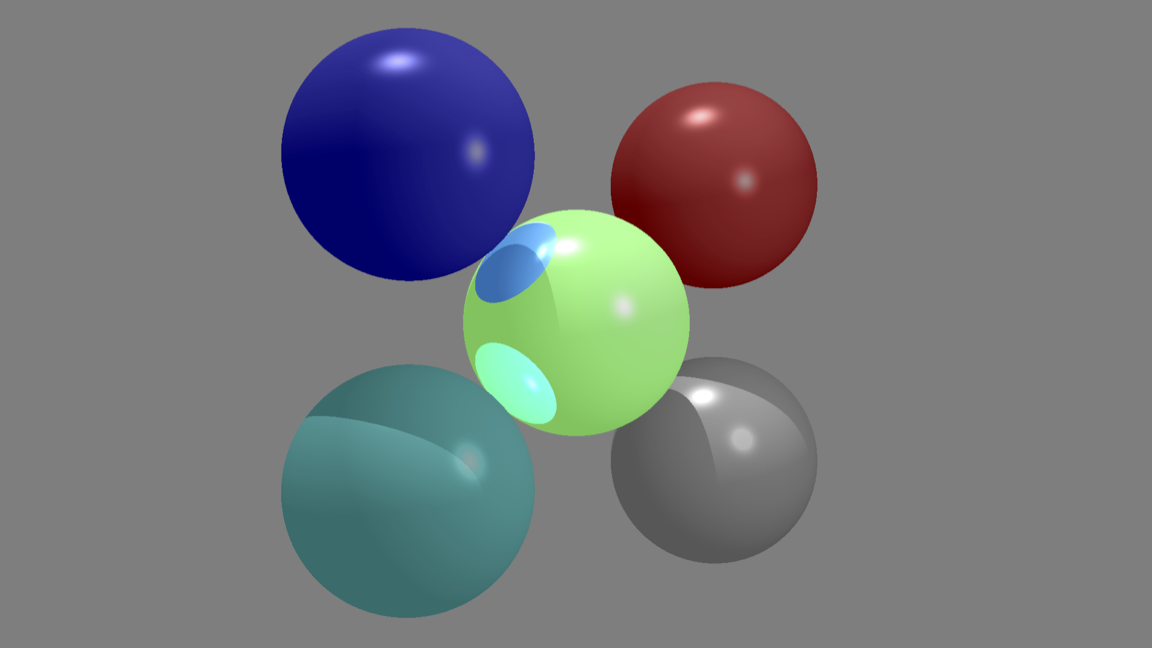
\includegraphics[scale=0.6]{raytrace}

\subsubsection{Run Time}

\section{\emph{Limitations}}
Currently there are a few limitations to FCL. They are connected to the limitations
that plague many other GPGPU platforms. Most notably is that gbuffers and glists
cannot be dynamically sized.

- glists and gbuffers are homogenous and one dimensional
- glists and gbuffers cannot be dynammically sized
- filter not possible because of lack of dynamically sized lists
- procedures cannot be used as input or output types
- lists cannot be output types
- parallelization is only work it if alg is O(n squared) and above or n is extrememly large


\section{\emph{Future work}}

\section{\emph{Conclusion}}

\section{\emph{Related work}}

Here is an example of a citation \cite{patrascu2010power}.

\section{\emph{Bibliography}}

\bibliographystyle{abbrv}

\bibliography{gpu-dsel-paper}

\end{document}
